%% PART 2 : SERIOUS GAMES
\subsection{Les Serious Games}
Definition.
	%% A Serious Games et Théories Comportementales 
	\subsubsection{Serious Games et Théories Comportementales }
			\paragraph{}
Les jeux vidéo sérieux se présentent comme un potentiel médiateur dans la modification des habitudes comportementales en permettant d’inclure des connaissances pratiques dans un modèle ludique apprécié. Il est possible d’y mettre en place des procédures de changement comme l’établissement d’objectifs ou la modélisation et le développement de compétences dans un environnement attrayant, significatif et immersif [Baranowski et al, 2008]. \\
Les jeux vidéo promeuvent les interactions sociales et d’apprentissage [Wideman et all, 2008], créent un environnement où les actions du joueur ont un effet [Gee, 2004] , encouragent la résolution de problèmes [Gee, 2004] et renforcent la compréhension en créant des situations de réflexion ou en aidant le joueur dans ses objectifs [Gee, 2004]. Enfin, les jeux sérieux pour la santé sont fait pour distraire le joueur tout en l’éduquant, en l’entrainant ou en changeant ses comportements [Stokes, 2005].

		\subsubsection*{Théories comportementales}
Le comportement est la résultante d’influences multiples, rendant ainsi souvent les personnes réfractaires au changement [Baranowski, Lin \& al, 1997]. Le comportement doit alors être considéré comme un mécanisme complexe découlant de l’enchaînement de plusieurs étapes. Ainsi, plutôt que de chercher à impacter directement le comportement, les experts comportementaux valorisent une action sur ces facteurs intermédiaires, appelés médiateurs. Changer ces médiateurs permet de changer le comportement [Baranowski, Lin \& al 1997].
\paragraph{}Plusieurs grandes théories comportementales existent~:
\begin{itemize}
	\item la théorie d’inoculation comportementale [McGuire, 1961]
	\item la théorie socio-cognitive [Bandura, 1986]
	\item la théorie de l’auto- étermination [Ryan \& Deci, 2000]
	\item la théorie de l’immersion [Green \& Brock, 2000]
\end{itemize}

\paragraph{}De ces théories, l’on peut alors identifier un certains nombre de ces facteurs médiateurs tels que : l’immersion, l’attention, l’auto-régulation, le développement de compétences, la motivation interne et externe, l’autonomie ou encore le sentiment de compétence. La science du comportement fournit aussi des techniques qui facilitent le changement comportemental, et propose d’utiliser ces facteurs dans les média de divertissement tel que le jeu vidéo.\\
Le modèle : "Elaboration Likelihood Model" [Petty \& Cacioppo, 1986] soutient ainsi que des personnages crédibles, attrayants et sympathiques sont plus susceptibles d’être persuasifs que les autres et peuvent donc servir d’intermédiaires pour véhiculer un message. \\
La théorie d’inoculation comportementale [McGuire, 1961] met en garde contre une possible contre-productivité en identifiant et en réfutant les menaces potentielles à l’accomplissement des objectifs du changement désiré.\\
La théorie socio-cognitive [Bandura, 1986] préconise l’établissement d’objectifs et le développement de compétences comme paramètres importants dans le changement comportemental.\\
Enfin, les théories socio-cognitive [Bandura, 1986] et d’auto-détermination [Ryan \& Deci, 2000] mettent toutes deux l’accent sur l’importance du feedback pour guider et mettre en forme le comportement durant le processus de changement.	

		\subsubsection*{Utilisation de la théorie pour un Serious Game éducatif}
			\paragraph{Identification \\ \quad}
Fait référence aux feedbacks ou aux conseils qui sont \emph{personnalisés} afin de mieux toucher le joueur [Kreuter, Strecher \& Glassman, 1999]. 
			\paragraph{Mini-jeux de connaissances \\ \quad}
Des connaissances pratiques et théoriques spécifiques sont un élément nécessaire, mais pas suffisant, d’une modification des habitudes comportementales [Bandura, 1986]. Ces mini-jeux peuvent être explicites (dans un mode à part) ou correspondrent aux boucles micro du gameplay.
			\paragraph{Ajustement des objectifs \\ \quad}
C’est un processus complexe qui permet à la fois de définir un objectif et les manières de l’atteindre [Gollwitzer, 1999], en prenant en considération les capacités et valeurs personnelles pour les lier à son objectif [Ryan \& Deci, 2000]. Parce que l’autonomie améliore la motivation personnelle [Ryan \& Deci, 2000], proposer et permettre au joueur de réaliser ses propres choix ou de paramétrer ses objectifs est donc conseillé.
			\paragraph{Résolution de problèmes \\ \quad}
Bien que les difficultés et obstacles interfèrent de premier abord dans la réalisation de ses objectifs, arriver à les surmonter est un moteur de motivation puissant [Frauenknecht \& Black, 1995]. Le joueur doit prévoir ces difficultés et mettre en place un plan pour arriver à les dépasser. Ces solutions doivent paraitre réalisables et plausibles pour ne pas décourager le joueur [Elaboration Likelihood Model : Petty \& Cacioppo, 1986].
			\paragraph{Exposition des motivations \\ \quad}
La théorie de l’auto-détermination [Ryan \& Deci, 2000] indique que la motivation personnelle est d’autant plus importante que la personne voit le lien entre son comportement et des choses importantes pour elle, comme une valeur qui lui est chère.
			\paragraph{Revue des objectifs et du travail accompli\\ \quad}
Cette activité renforce le sentiment d’accomplissement personnel et augmente l’auto-efficacité [Bandura, 1986].
			\paragraph{Feedback \\ \quad}
Un feedback bien conçu renforce l’efficacité personnelle [Schuk, 1986] et le sentiment de compétence. [Ryan \& Deci, 2000]
			
\paragraph{}
Pour vérifier l'application de ces théories sur un cas pratique, [Thompson et al] ont participé à la création d'un Serious Game~: DIAB. DIAB est un jeu vidéo divertissant, mais sérieux et se basant sur ces concepts théoriques, conçu pour réduire les risques de diabète de type 2 et d’obésité infantile. Il émerge de cette expérience que les jeux sérieux fondés sur une base théorique peuvent être efficaces pour parvenir à un changement à la fois dans le régime alimentaire et l’activité physique. Peu est encore connu dans le domaine, mais il en sort que les mécanismes et processus de changements comportementaux ont aussi leur place dans les jeus sérieux  et peuvent permettre d'améliorer l'efficacité de ces derniers. Cette expérience décrit aussi comment les experts du divertissement et du comportement peuvent allier leurs talents respectifs pour créer un jeu divertissant basé sur un socle théorique. 
	%% Apprentissage et propriétés des jeux vidéo
	\subsubsection{Apprentissage et propriétés (ou attributs) des jeux vidéo}
			\subsubsection*{Référence Wilson}
			Définir les attributs principaux, quitte à balancer le tableau réduit anglais.
			
			\subsubsection*{Référence GEE}

			\subsubsection*{Référence Thompson}						
			
	%% Serious games thérapeutiques
	\subsubsection{Serious games pour la santé}

\begin{figure}
Succinte explication du lien entre mes composantes. Vérifier que ca se trouve avec le reste et pas en fin de document.
	\centering
	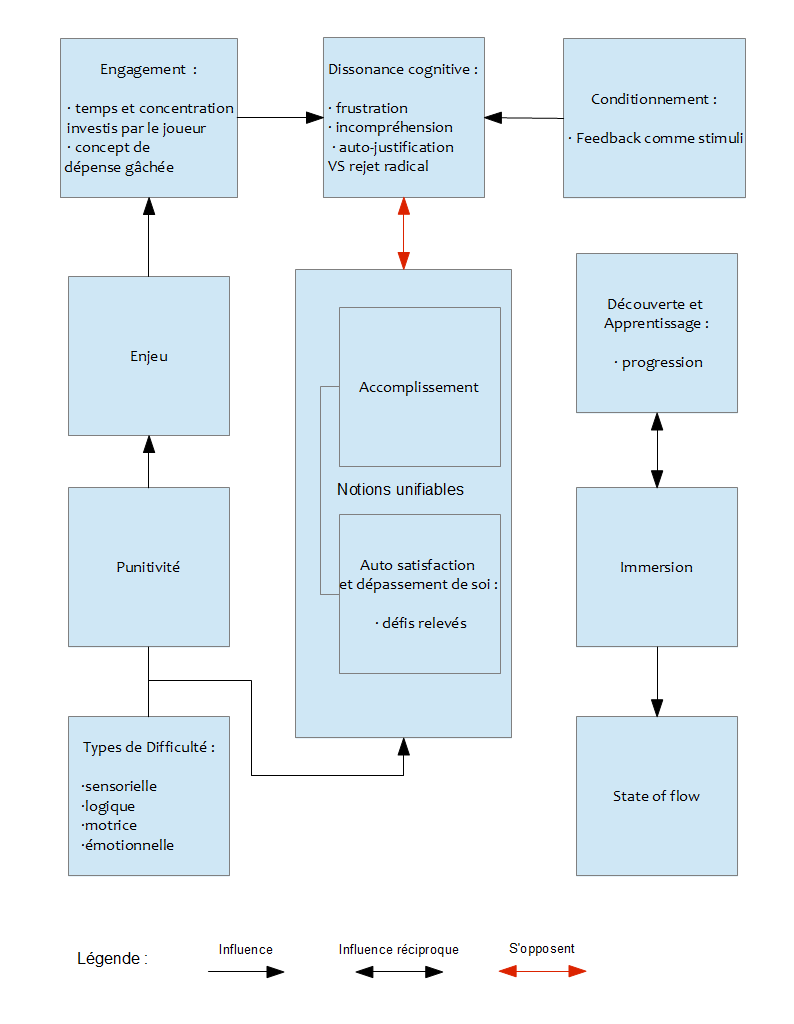
\includegraphics[height=19.6cm]{images/lien_theories}
	\caption{Relation entre les principaux ressorts psychologiques d'un jeu vidéo}
	\label{lien_theories}
\end{figure}